\section{RQ1: Scaling Without Synchronization}
\label{sec:rq1}

The main campaign ran 3 environments $\times$ (9 workload configurations
$\times$ $N \in \{1,2,4,6,7,8\}$ + 5 sequential references) $\times$ 30
runs = 5310 runs in one random order (seed 2026112201), in 14.0 hours.
Tables~\ref{tab:times}, \ref{tab:speedup} and~\ref{tab:efficiency} give the
time, the speedup and the efficiency of every cell;
Figures~\ref{fig:speedup} and~\ref{fig:efficiency} draw them.

\begin{figure}[tbp]
\centering
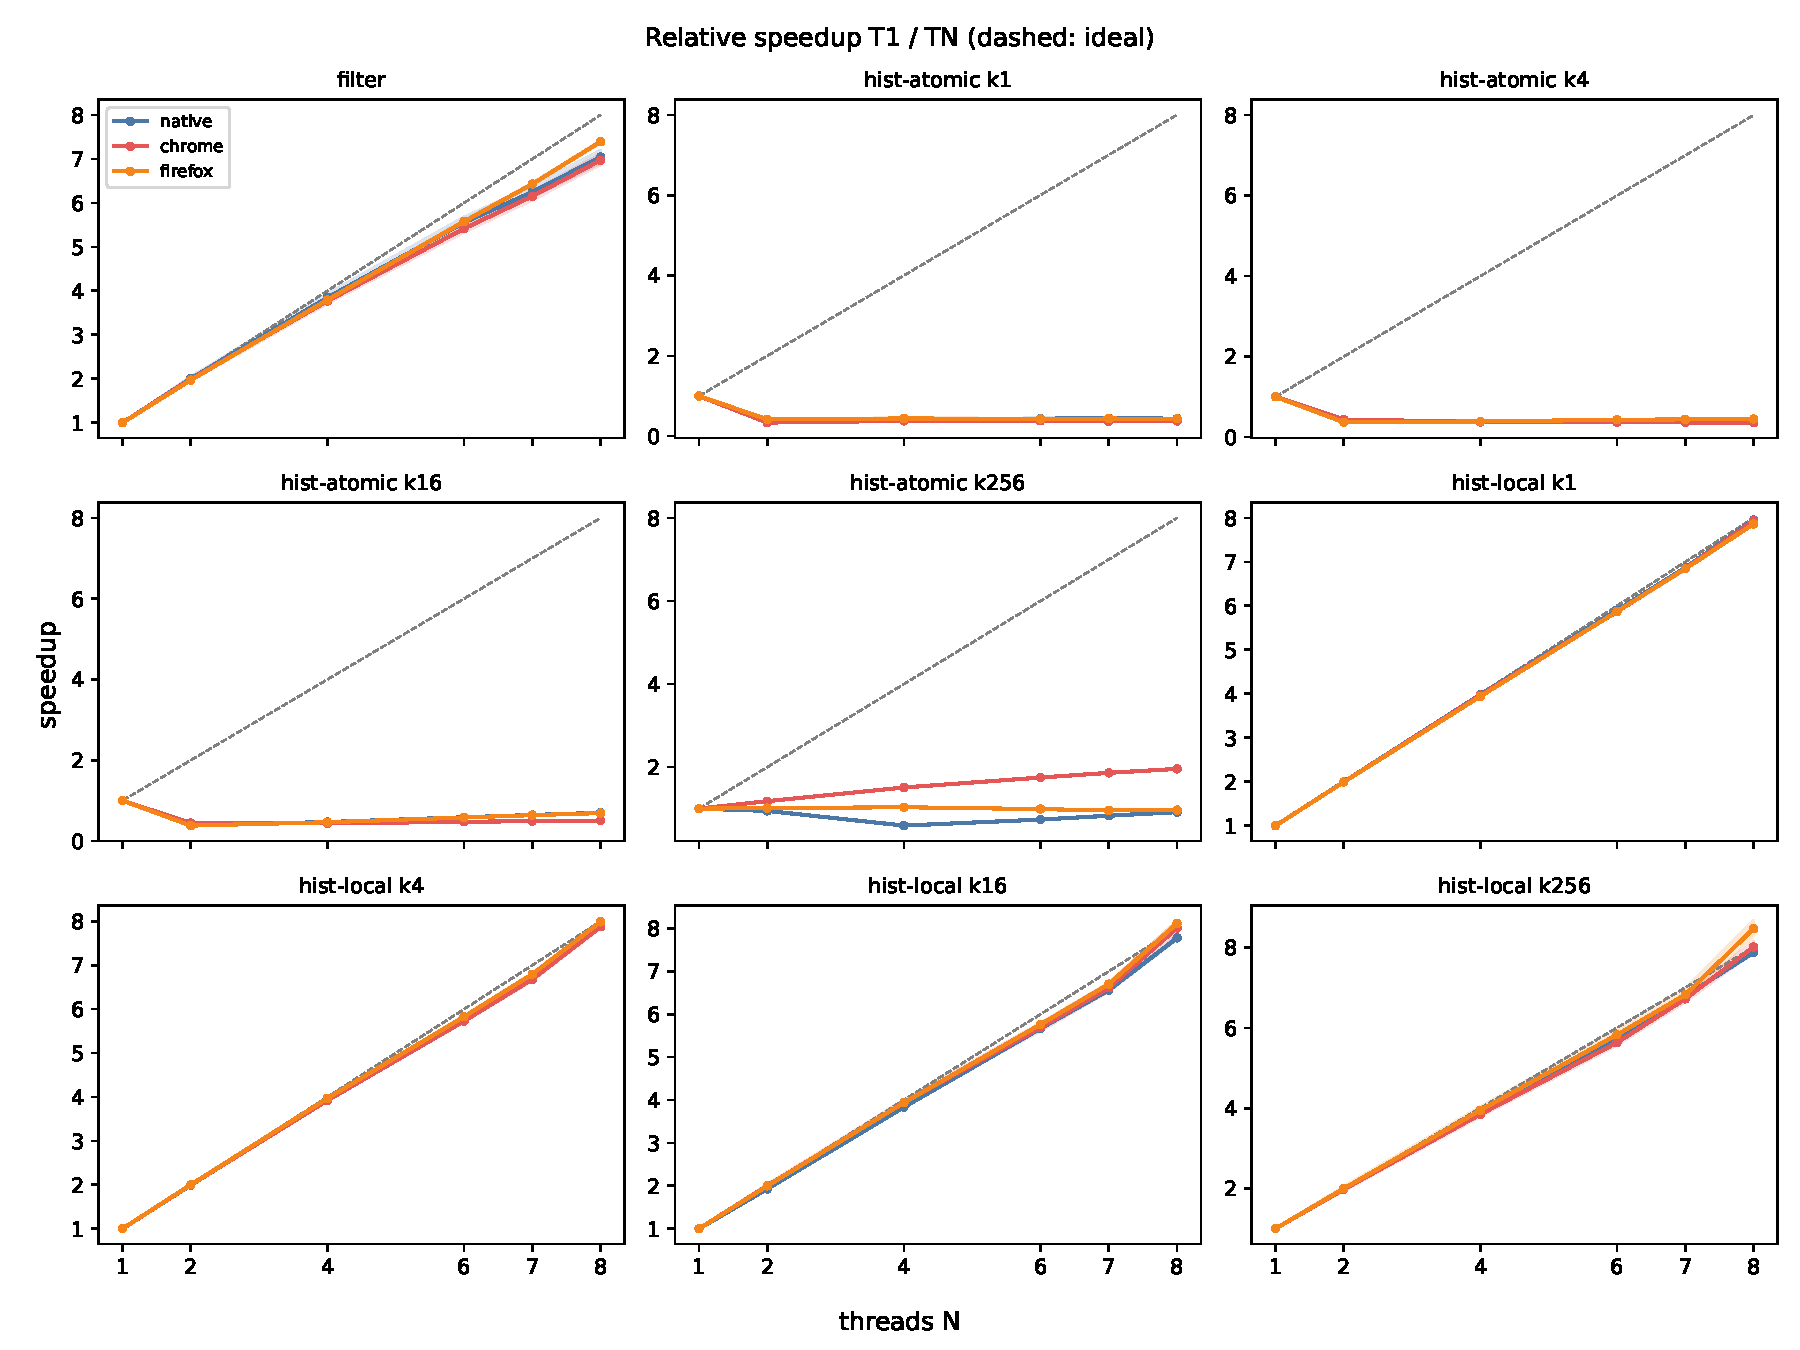
\includegraphics[width=\linewidth]{../figures/campaign-speedup.pdf}
\caption{Relative speedup against $N$ per workload (30 runs per point,
bands: 95\% CI; dashed: ideal).}
\Description{Speedup against thread count, one panel per workload, for native, Chrome and Firefox.}
\label{fig:speedup}
\end{figure}

\begin{figure}[tbp]
\centering
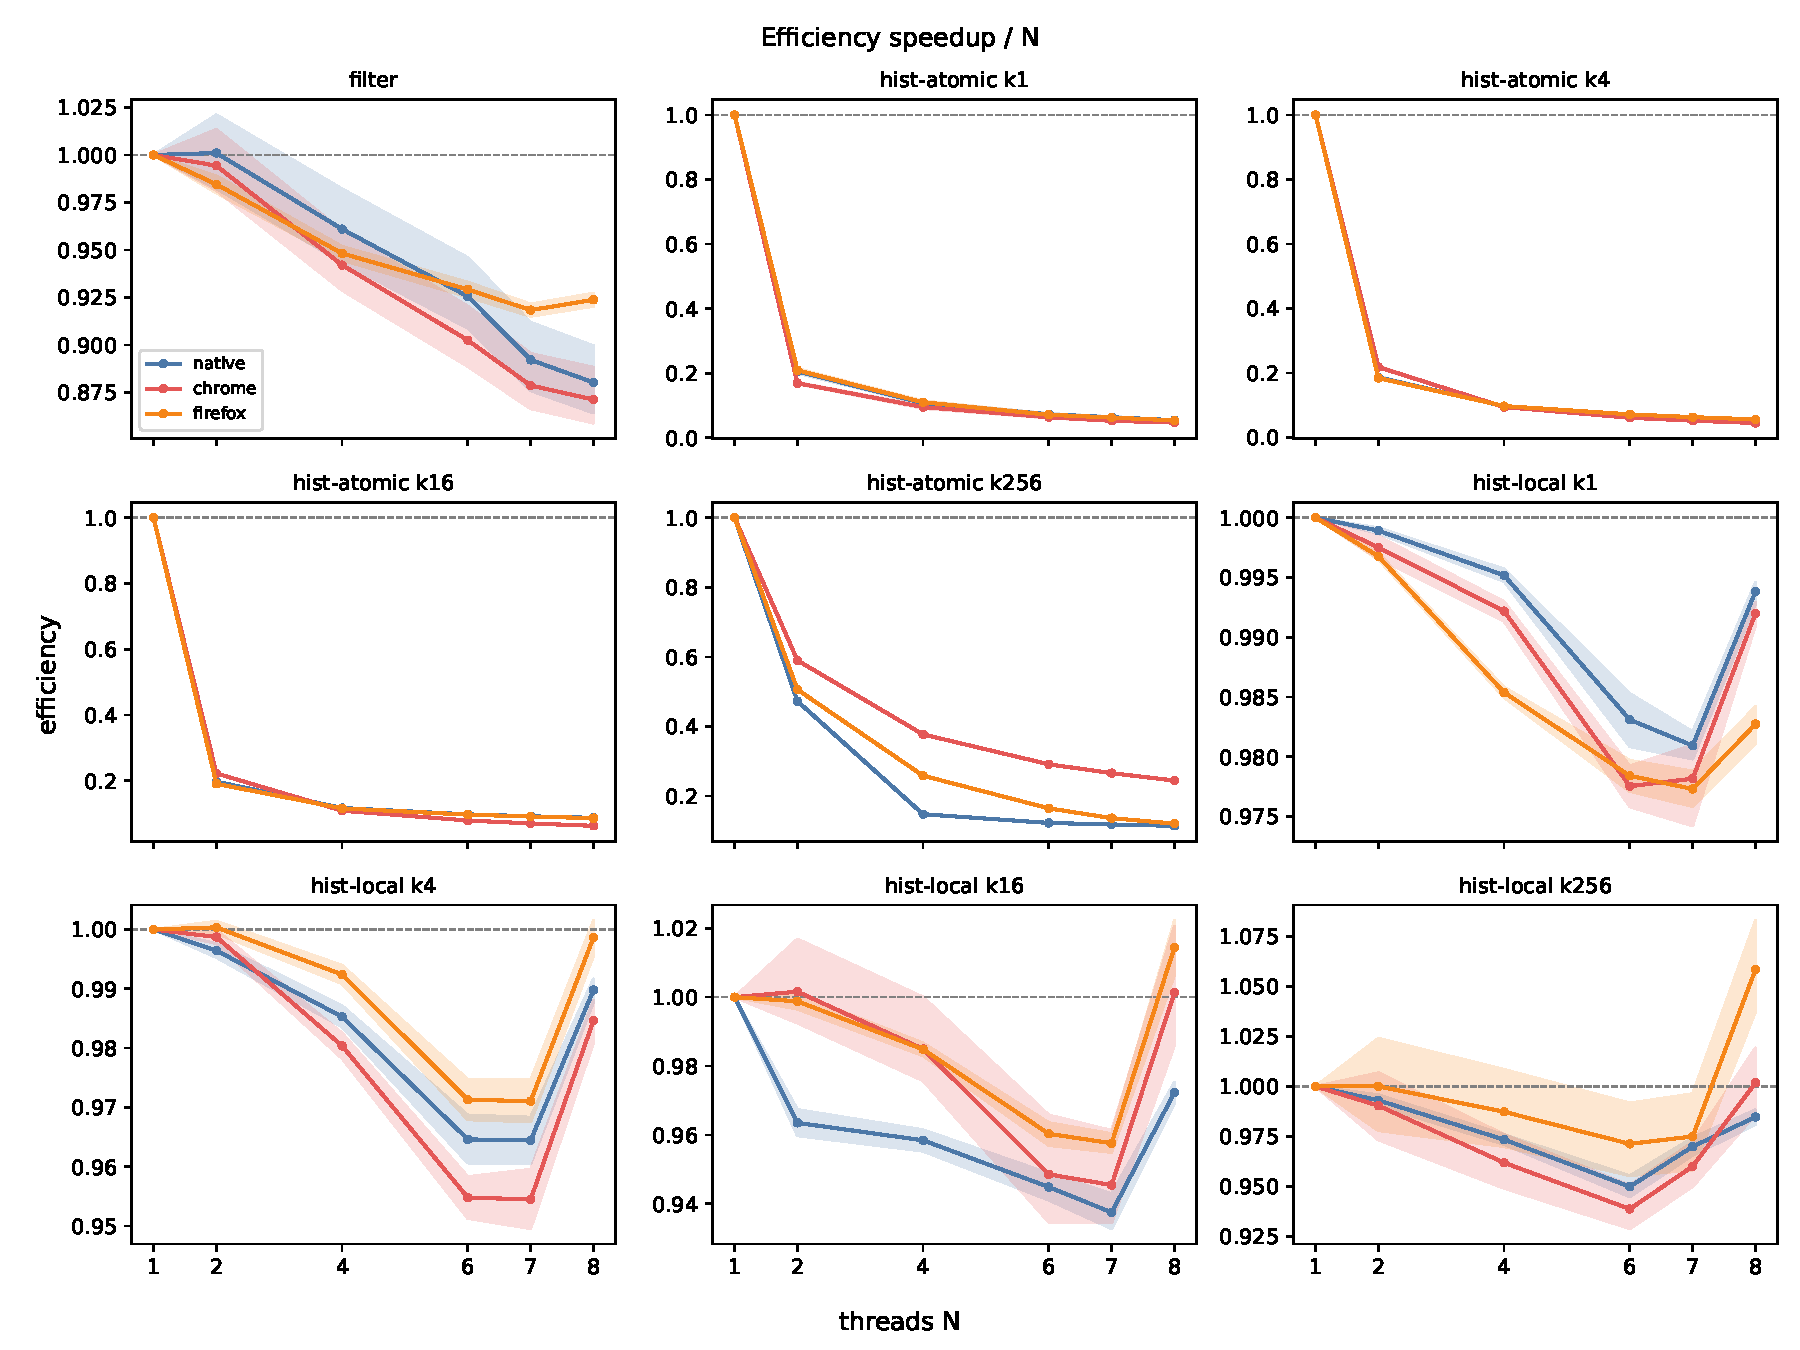
\includegraphics[width=\linewidth]{../figures/campaign-efficiency.pdf}
\caption{Efficiency $S_N/N$ against $N$ per workload (bands: 95\% CI).}
\Description{Efficiency against thread count, one panel per workload, for native, Chrome and Firefox.}
\label{fig:efficiency}
\end{figure}

\subsection{The primary result}

The filter reaches a speedup of 6.96 at $N=8$ natively (95\% CI [6.94,
6.97]), 6.92 in Chrome [6.89, 6.96] and 7.34 in Firefox [7.24, 7.42]: an
efficiency of 0.869, 0.865 and 0.917. The two primary RQ1 contrasts
(Table~\ref{tab:primary}) are the ratios of those speedups to native's:
\begin{itemize}[leftmargin=1.5em]
\item \emph{Chrome}: 0.996, 99.5\% CI [0.987, 1.004], not rejected
(Holm-adjusted $p = 0.28$). Chrome's filter speedup is within $-1.3$\% to
$+0.4$\% of native's. A non-rejection is not proof of equality; the
interval is the bound.
\item \emph{Firefox}: 1.055, 99.5\% CI [1.034, 1.072], rejected. Firefox's
speedup is 5.5\% higher than native's, from a slower baseline: its filter
takes 30.8~ms on one thread against 22.6~ms natively, and 4.20 against
3.25~ms on eight. Section~\ref{sec:why-rq1} explains why a slower loop
scales better here.
\end{itemize}

\begin{table}[htbp]
\caption{The ten primary contrasts at $N=8$: effect, 95\,\% interval, Bonferroni 99.5\,\% interval, bootstrap $p$, Holm-adjusted $p$ and the decision at $\alpha=0.05$.}\label{tab:primary}
\centering\footnotesize
\begin{tabular}{lllccrrl}
\toprule
RQ & Browser & Cell & Effect [95\,\%] & [99.5\,\%] & $p$ & Holm $p$ & Rejected \\
\midrule
RQ1 & Chrome & filter & 0.9955 [0.9896, 1.002] & [0.9868, 1.004] & 0.1416 & 0.2832 & no \\
RQ1 & Firefox & filter & 1.055 [1.041, 1.067] & [1.034, 1.072] & 0.0001 & 0.001 & yes \\
RQ2 & Chrome & atomic, $k$=1 & 2.259 [2.157, 2.365] & [2.11, 2.406] & 0.0001 & 0.001 & yes \\
RQ2 & Chrome & atomic, $k$=4 & 1.771 [1.754, 1.787] & [1.746, 1.793] & 0.0001 & 0.001 & yes \\
RQ2 & Chrome & atomic, $k$=16 & 1.425 [1.408, 1.442] & [1.399, 1.451] & 0.0001 & 0.001 & yes \\
RQ2 & Chrome & atomic, $k$=256 & 0.4159 [0.4096, 0.4222] & [0.4072, 0.4251] & 0.0001 & 0.001 & yes \\
RQ2 & Firefox & atomic, $k$=1 & 1.01 [0.9724, 1.049] & [0.9573, 1.067] & 0.5994 & 0.5994 & no \\
RQ2 & Firefox & atomic, $k$=4 & 0.9691 [0.9597, 0.9788] & [0.9555, 0.9827] & 0.0001 & 0.001 & yes \\
RQ2 & Firefox & atomic, $k$=16 & 0.8311 [0.824, 0.8385] & [0.8208, 0.8417] & 0.0001 & 0.001 & yes \\
RQ2 & Firefox & atomic, $k$=256 & 0.7965 [0.7864, 0.8058] & [0.782, 0.8089] & 0.0001 & 0.001 & yes \\
\bottomrule
\end{tabular}
\end{table}


The local histogram, which also has no shared write, reaches 7.83 to 8.48
at $N=8$ in every environment and at every $k$ (efficiency 0.98 to 1.06).
The exploratory speedup ratios of every cell are in
Table~\ref{tab:rq1-ratios}: for the local histogram they stay between 0.99
and 1.07 at $N=8$. Two features of these curves are taken up later: the
efficiency above 1 in Firefox at $k \geq 16$ (speedups of 8.26 and 8.48,
Section~\ref{sec:why-superlinear}), and a dip of the efficiency at six and
seven threads that recovers at eight, in every environment
(Section~\ref{sec:dip}).

\subsection{Absolute time: a constant factor}

A speedup compares an environment with itself.
Table~\ref{tab:absolute} and Figure~\ref{fig:absolute} give the time in the
browser over the native time at the same $N$. On one thread WASM is slower
for the filter (Chrome 1.172 times native [1.167, 1.177], Firefox 1.363
[1.356, 1.372]) and for the local histogram at $k \geq 16$ (1.23 to 1.27
times), and within 7\% at $k \leq 4$. The ratio does not grow with $N$:
for the filter at eight threads it is 1.177 in Chrome and 1.292 in Firefox.
WASM threads cost a constant factor in time, not scalability.

One cell goes the other way: at $k=1$ Chrome's local histogram is 2.7\%
\emph{faster} than native (0.973 [0.972, 0.974]). With every pixel on one
counter the loop is a chain through memory, bound by store-to-load
forwarding and not by throughput; LLVM uses one read-modify-write
instruction per pixel (\code{inc} on memory) and V8 a load, an add and a
store. An investigation on the first build timed both sequences by hand in
a native microbenchmark and reproduced the campaign's difference within
about 1\%. It is evidence from an earlier build, and it matches the
listings of v3 (Section~\ref{sec:engine-code}); the point for the reader is
that the engine's code generator is part of what is measured, in both
directions.

\begin{figure}[tbp]
\centering
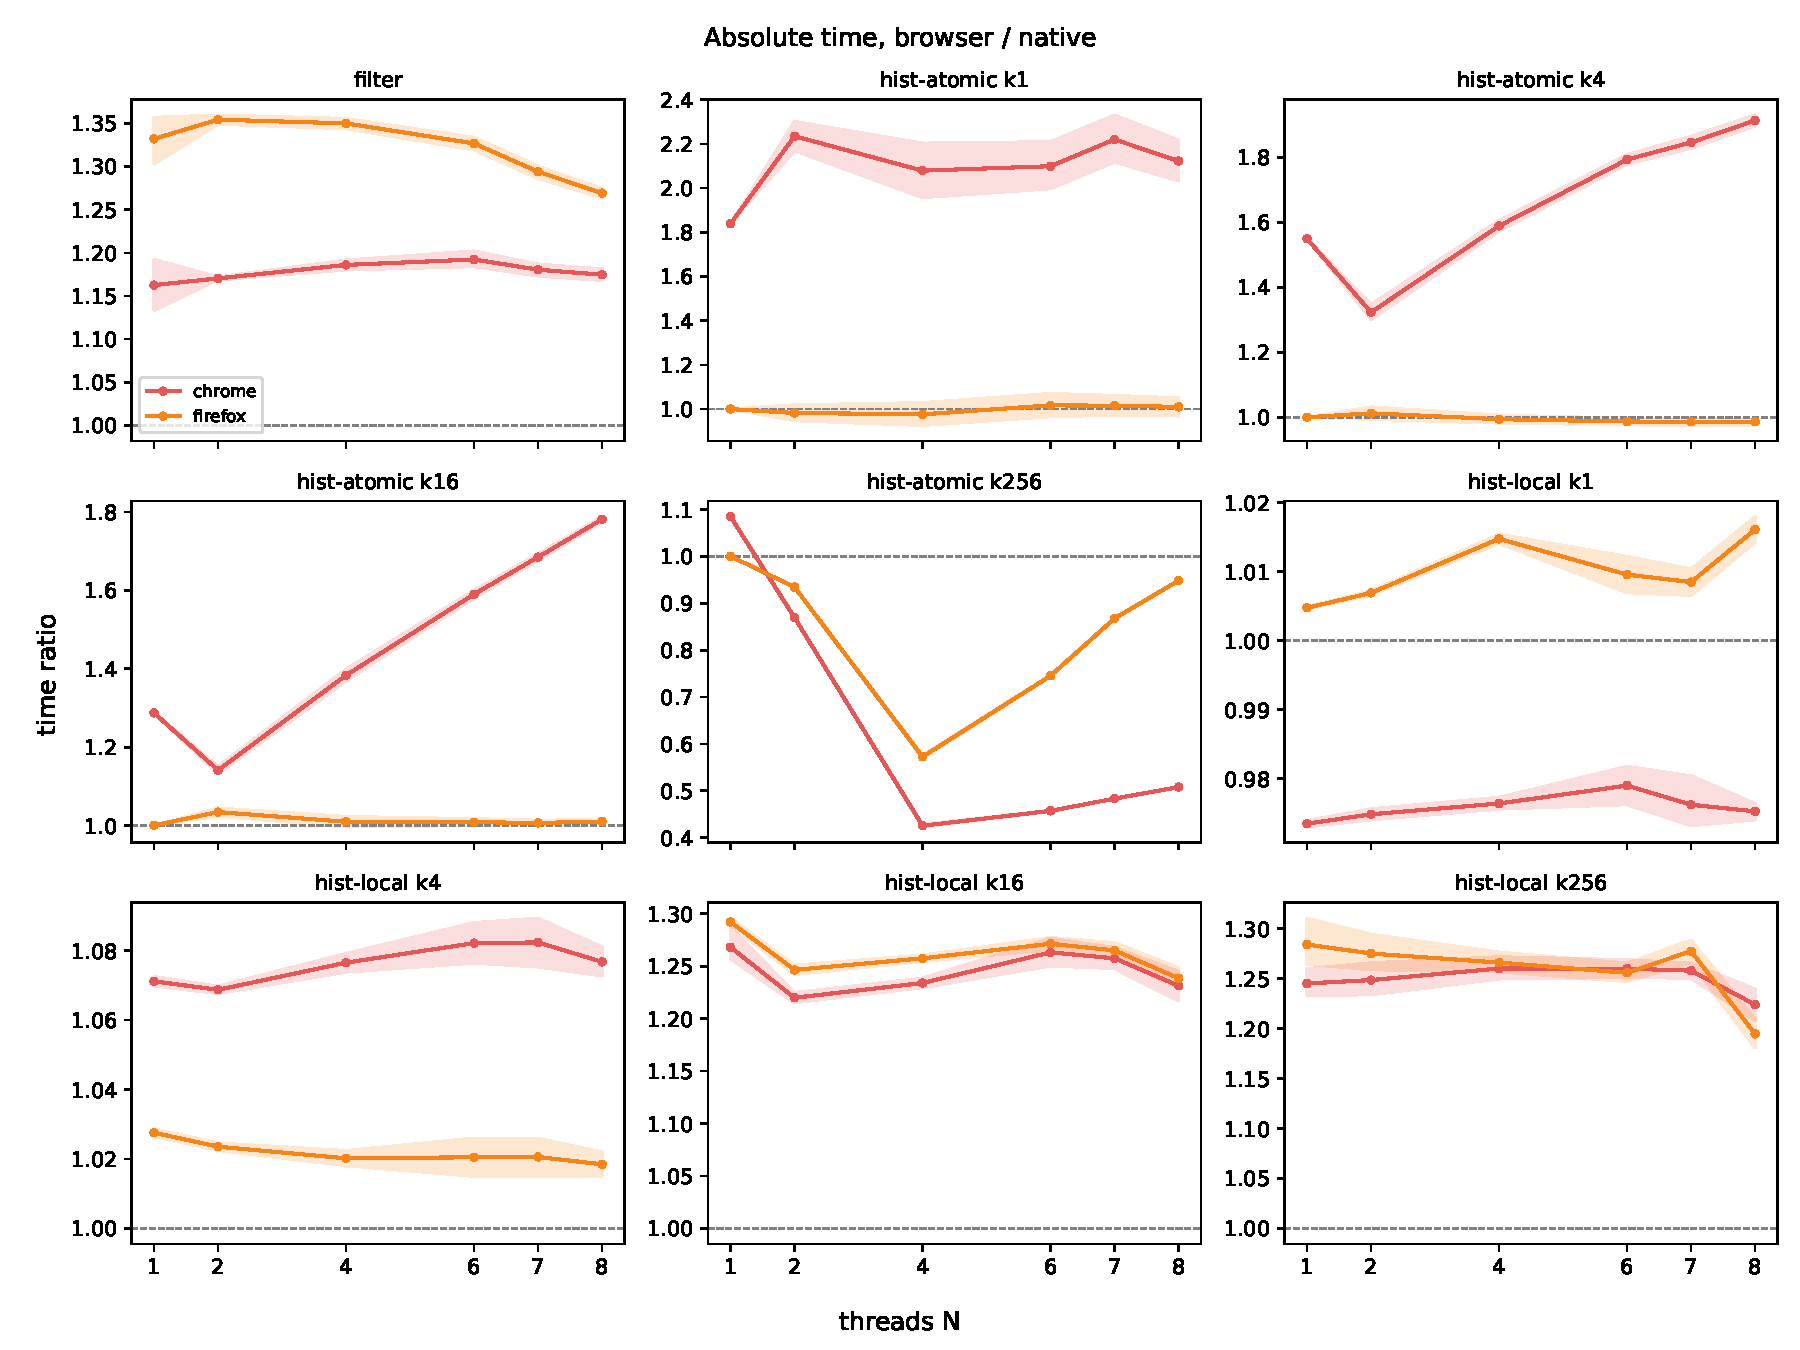
\includegraphics[width=\linewidth]{../figures/campaign-absolute.pdf}
\caption{Absolute time of one iteration against $N$ per workload and
environment.}
\Description{Absolute time against thread count per workload for the three environments.}
\label{fig:absolute}
\end{figure}

\subsection{Is the speedup inflated by a slow baseline?}
\label{sec:sequential}

Relative speedup divides by the time of a pool of one thread. If that pool
were slow compared with code that has no pool at all, every speedup would
be inflated. The sequential references answer it
(Table~\ref{tab:sequential}): the sequential kernel takes between 0.957 and
1.072 times the time of the pool of one thread, that is, the pool costs
between 7\% less and 5\% more than sequential code, in every environment.
For the filter the pool costs under 1\% natively and in Chrome and 2.5\%
in Firefox. Against the sequential reference the filter still reaches 6.90,
6.86 and 7.15 at eight threads, and the local histogram's speedup above 8
in Firefox is still there (8.09 and 8.12 at $k=16$ and 256). Natively the
sequential histogram and one task of the local histogram are the same
machine-code loop.

\begin{table}[htbp]
\caption{Sequential references: time of the kernel without Rayon in ms, the pool of one thread against it ($T_{seq}/T_1$ with its 95\,\% interval; 1 means the pool costs nothing), and the speedup of eight threads against it.}\label{tab:sequential}
\centering\scriptsize
\begin{tabular}{lrcrrcrrcr}
\toprule
 & \multicolumn{3}{c}{Native} & \multicolumn{3}{c}{Chrome} & \multicolumn{3}{c}{Firefox} \\
Workload & $T_{seq}$ & $T_{seq}/T_1$ & $T_{seq}/T_8$ & $T_{seq}$ & $T_{seq}/T_1$ & $T_{seq}/T_8$ & $T_{seq}$ & $T_{seq}/T_1$ & $T_{seq}/T_8$ \\
\midrule
filter & 22.413 & 0.9917 [0.9911, 0.9922] & 6.898 & 26.237 & 0.9906 [0.9854, 0.9958] & 6.859 & 30.035 & 0.9749 [0.9627, 0.986] & 7.152 \\
local, $k$=1 & 155.1 & 1.001 [1.001, 1.001] & 7.967 & 153.8 & 1.02 [1.019, 1.021] & 8.092 & 152.8 & 0.9815 [0.9724, 0.9885] & 7.725 \\
local, $k$=4 & 42.704 & 0.9945 [0.9939, 0.9951] & 7.907 & 43.916 & 0.9563 [0.9531, 0.9582] & 7.544 & 42.655 & 0.9703 [0.9648, 0.9747] & 7.78 \\
local, $k$=16 & 27.695 & 0.9674 [0.9596, 0.9743] & 7.607 & 38.178 & 1.072 [1.062, 1.08] & 8.395 & 35.676 & 0.979 [0.9768, 0.9813] & 8.086 \\
local, $k$=256 & 26.593 & 0.9816 [0.9741, 0.987] & 7.785 & 33.964 & 1.018 [1.003, 1.03] & 8.149 & 32.993 & 0.9566 [0.9363, 0.9728] & 8.116 \\
\bottomrule
\end{tabular}
\end{table}


Table~\ref{tab:throughput} gives the same data as nanoseconds per pixel and
as the \emph{absolute} speedup, the native one-thread time over the time of
the environment at $N$: on eight threads the filter is 6.96 times faster
than one native thread natively, 5.91 times in Chrome and 5.38 times in
Firefox.

\subsection{Fork-join: what does not divide with the work}
\label{sec:forkjoin}

The constant factor divides with the work; the cost of starting and ending
a parallel region does not. The calibration of every run measures it
(Table~\ref{tab:fork-join}). With the workers awake (warm), an empty
\code{broadcast} at $N=8$ takes 110~\textmu s in Chrome and 60~\textmu s in
Firefox against 7.9~\textmu s natively (medians over 270 runs of the
per-run median), and an empty parallel iterator 25, 20 and 5.4~\textmu s.
The means are larger (164, 91 and 46~\textmu s for the broadcast), so the
distribution has a tail. Three cautions go with these numbers:
\begin{itemize}[leftmargin=1.5em]
\item \emph{Resolution.} With a 20~\textmu s clock, Firefox's warm values
are multiples of 20 and read 0 at $N \leq 4$; Chrome's are multiples of 5.
Twenty samples per probe do not resolve them better.
\item \emph{A step at $N=8$.} Natively the broadcast takes 1.8 to
3.1~\textmu s up to $N=7$ and 7.9 at $N=8$, and Chrome's goes from 10 to
110. At eight threads the coordinating thread shares the eight cores with
eight workers; that this is the cause was not tested.
\item \emph{Cold depends on what ran before.} After a pause the workers are
asleep, as before a measured iteration. In filter runs the cold broadcast
at $N=8$ takes 205~\textmu s natively, 460 in Chrome and 270 in Firefox; in
histogram runs 31 to 34, 65 and 80 to 85, so that Chrome's cold call is
cheaper than its warm one there. The pause is as long as the workload's
checksum, which differs between workloads; the cause is not established.
\end{itemize}
With iterations of milliseconds these costs are amortized (0.33\% of $T_8$
natively at 8192$^2$, 1.4\% in Firefox and 2.7\% in Chrome with the warm
cost, Section~\ref{sec:cutoff}); with regions under a millisecond they are a
large share of the time.

\subsection{Karp-Flatt}

Table~\ref{tab:karp-flatt} gives the serial fraction that Amdahl's law
would need to explain each speedup. For the filter at $N=8$ it is 0.021
natively, 0.022 in Chrome and 0.013 in Firefox, and it does not fall as $N$
grows (natively 0.018, 0.019, 0.021 at $N=2$, 4, 8). But the timed region
of the filter has no serial part: every row is processed in parallel and
nothing else is timed. So $e$ here is not serial code, it is a cost of
running in parallel, and Section~\ref{sec:why-rq1} attributes about half of
it natively to the cores' own slower work on shared memory. For the local
histogram $e$ is between $-0.008$ and $0.013$ from $N=4$ on.

{\small
\begin{longtable}{llrrr}
\caption{Main campaign: time of one iteration in ms (geometric mean over 30 runs of the per-run median of 10 measured iterations).}\label{tab:times} \\
\toprule
Workload & $N$ & Native & Chrome & Firefox \\
\midrule
\endfirsthead
\toprule
Workload & $N$ & Native & Chrome & Firefox \\
\midrule
\endhead
\bottomrule
\endfoot
filter & 1 & 22.601 & 26.486 & 30.808 \\
filter & 2 & 11.502 & 13.505 & 15.641 \\
filter & 4 & 5.979 & 7.111 & 8.146 \\
filter & 6 & 4.140 & 4.909 & 5.535 \\
filter & 7 & 3.658 & 4.350 & 4.814 \\
filter & 8 & 3.249 & 3.825 & 4.200 \\
\midrule
atomic, $k$=1 & 1 & 379.6 & 698.0 & 379.7 \\
atomic, $k$=1 & 2 & 901.0 & 2028.1 & 932.4 \\
atomic, $k$=1 & 4 & 842.0 & 1905.8 & 849.2 \\
atomic, $k$=1 & 6 & 838.0 & 1868.5 & 869.0 \\
atomic, $k$=1 & 7 & 885.4 & 1876.6 & 900.3 \\
atomic, $k$=1 & 8 & 856.3 & 1888.8 & 878.5 \\
\midrule
atomic, $k$=4 & 1 & 379.6 & 588.7 & 379.7 \\
atomic, $k$=4 & 2 & 1009.8 & 1362.6 & 1025.0 \\
atomic, $k$=4 & 4 & 976.8 & 1546.2 & 970.8 \\
atomic, $k$=4 & 6 & 900.9 & 1613.4 & 885.0 \\
atomic, $k$=4 & 7 & 870.8 & 1631.9 & 866.4 \\
atomic, $k$=4 & 8 & 863.6 & 1648.4 & 849.6 \\
\midrule
atomic, $k$=16 & 1 & 379.5 & 488.5 & 379.8 \\
atomic, $k$=16 & 2 & 957.3 & 1099.9 & 989.7 \\
atomic, $k$=16 & 4 & 805.7 & 1124.1 & 819.7 \\
atomic, $k$=16 & 6 & 646.1 & 1029.5 & 651.1 \\
atomic, $k$=16 & 7 & 588.6 & 992.7 & 593.2 \\
atomic, $k$=16 & 8 & 544.0 & 968.4 & 548.0 \\
\midrule
atomic, $k$=256 & 1 & 379.6 & 411.9 & 379.8 \\
atomic, $k$=256 & 2 & 401.5 & 349.0 & 375.2 \\
atomic, $k$=256 & 4 & 639.7 & 273.9 & 368.2 \\
atomic, $k$=256 & 6 & 515.8 & 235.2 & 383.9 \\
atomic, $k$=256 & 7 & 458.1 & 221.3 & 396.7 \\
atomic, $k$=256 & 8 & 414.6 & 210.4 & 393.0 \\
\midrule
local, $k$=1 & 1 & 154.9 & 150.7 & 155.6 \\
local, $k$=1 & 2 & 77.581 & 75.511 & 78.060 \\
local, $k$=1 & 4 & 38.929 & 37.992 & 39.485 \\
local, $k$=1 & 6 & 26.250 & 25.759 & 26.515 \\
local, $k$=1 & 7 & 22.562 & 21.981 & 22.752 \\
local, $k$=1 & 8 & 19.473 & 19.011 & 19.775 \\
\midrule
local, $k$=4 & 1 & 42.939 & 45.924 & 43.961 \\
local, $k$=4 & 2 & 21.481 & 22.940 & 21.958 \\
local, $k$=4 & 4 & 10.868 & 11.679 & 11.044 \\
local, $k$=4 & 6 & 7.382 & 8.005 & 7.554 \\
local, $k$=4 & 7 & 6.339 & 6.897 & 6.451 \\
local, $k$=4 & 8 & 5.401 & 5.822 & 5.482 \\
\midrule
local, $k$=16 & 1 & 28.627 & 35.616 & 36.440 \\
local, $k$=16 & 2 & 14.764 & 17.882 & 18.071 \\
local, $k$=16 & 4 & 7.395 & 9.051 & 9.188 \\
local, $k$=16 & 6 & 4.988 & 6.276 & 6.292 \\
local, $k$=16 & 7 & 4.297 & 5.390 & 5.412 \\
local, $k$=16 & 8 & 3.640 & 4.548 & 4.412 \\
\midrule
local, $k$=256 & 1 & 27.092 & 33.367 & 34.491 \\
local, $k$=256 & 2 & 13.597 & 16.742 & 17.268 \\
local, $k$=256 & 4 & 6.934 & 8.626 & 8.866 \\
local, $k$=256 & 6 & 4.752 & 5.930 & 5.976 \\
local, $k$=256 & 7 & 3.984 & 4.997 & 5.066 \\
local, $k$=256 & 8 & 3.416 & 4.168 & 4.065 \\
\end{longtable}
}

{\small
\begin{longtable}{llccc}
\caption{Main campaign: relative speedup $T_1/T_N$ with its 95\,\% bootstrap interval (30 runs per cell, geometric mean of the per-run medians).}\label{tab:speedup} \\
\toprule
Workload & $N$ & Native & Chrome & Firefox \\
\midrule
\endfirsthead
\toprule
Workload & $N$ & Native & Chrome & Firefox \\
\midrule
\endhead
\bottomrule
\endfoot
filter & 1 & 1.000 [1.000, 1.000] & 1.000 [1.000, 1.000] & 1.000 [1.000, 1.000] \\
filter & 2 & 1.965 [1.963, 1.967] & 1.961 [1.944, 1.977] & 1.970 [1.947, 1.991] \\
filter & 4 & 3.780 [3.774, 3.786] & 3.725 [3.702, 3.747] & 3.782 [3.727, 3.830] \\
filter & 6 & 5.459 [5.440, 5.475] & 5.396 [5.367, 5.424] & 5.566 [5.511, 5.619] \\
filter & 7 & 6.179 [6.166, 6.190] & 6.088 [6.055, 6.121] & 6.400 [6.341, 6.457] \\
filter & 8 & 6.955 [6.942, 6.969] & 6.924 [6.885, 6.964] & 7.336 [7.235, 7.422] \\
\midrule
atomic, $k$=1 & 1 & 1.000 [1.000, 1.000] & 1.000 [1.000, 1.000] & 1.000 [1.000, 1.000] \\
atomic, $k$=1 & 2 & 0.421 [0.412, 0.430] & 0.344 [0.338, 0.351] & 0.407 [0.394, 0.420] \\
atomic, $k$=1 & 4 & 0.451 [0.434, 0.468] & 0.366 [0.351, 0.382] & 0.447 [0.434, 0.461] \\
atomic, $k$=1 & 6 & 0.453 [0.437, 0.469] & 0.374 [0.360, 0.388] & 0.437 [0.423, 0.452] \\
atomic, $k$=1 & 7 & 0.429 [0.416, 0.444] & 0.372 [0.359, 0.386] & 0.422 [0.411, 0.435] \\
atomic, $k$=1 & 8 & 0.443 [0.431, 0.455] & 0.370 [0.357, 0.384] & 0.432 [0.421, 0.444] \\
\midrule
atomic, $k$=4 & 1 & 1.000 [1.000, 1.000] & 1.000 [1.000, 1.000] & 1.000 [1.000, 1.000] \\
atomic, $k$=4 & 2 & 0.376 [0.371, 0.381] & 0.432 [0.428, 0.436] & 0.370 [0.367, 0.374] \\
atomic, $k$=4 & 4 & 0.389 [0.386, 0.392] & 0.381 [0.378, 0.384] & 0.391 [0.388, 0.395] \\
atomic, $k$=4 & 6 & 0.421 [0.418, 0.425] & 0.365 [0.363, 0.367] & 0.429 [0.426, 0.432] \\
atomic, $k$=4 & 7 & 0.436 [0.433, 0.439] & 0.361 [0.359, 0.363] & 0.438 [0.435, 0.441] \\
atomic, $k$=4 & 8 & 0.440 [0.436, 0.443] & 0.357 [0.355, 0.359] & 0.447 [0.445, 0.449] \\
\midrule
atomic, $k$=16 & 1 & 1.000 [1.000, 1.000] & 1.000 [1.000, 1.000] & 1.000 [1.000, 1.000] \\
atomic, $k$=16 & 2 & 0.396 [0.393, 0.400] & 0.444 [0.441, 0.447] & 0.384 [0.381, 0.386] \\
atomic, $k$=16 & 4 & 0.471 [0.466, 0.476] & 0.435 [0.433, 0.437] & 0.463 [0.459, 0.468] \\
atomic, $k$=16 & 6 & 0.587 [0.585, 0.590] & 0.474 [0.473, 0.476] & 0.583 [0.580, 0.586] \\
atomic, $k$=16 & 7 & 0.645 [0.642, 0.647] & 0.492 [0.491, 0.494] & 0.640 [0.637, 0.643] \\
atomic, $k$=16 & 8 & 0.698 [0.695, 0.700] & 0.504 [0.503, 0.506] & 0.693 [0.691, 0.696] \\
\midrule
atomic, $k$=256 & 1 & 1.000 [1.000, 1.000] & 1.000 [1.000, 1.000] & 1.000 [1.000, 1.000] \\
atomic, $k$=256 & 2 & 0.945 [0.945, 0.946] & 1.180 [1.179, 1.180] & 1.012 [1.012, 1.012] \\
atomic, $k$=256 & 4 & 0.593 [0.589, 0.597] & 1.504 [1.499, 1.509] & 1.031 [1.030, 1.033] \\
atomic, $k$=256 & 6 & 0.736 [0.734, 0.738] & 1.751 [1.747, 1.755] & 0.989 [0.988, 0.991] \\
atomic, $k$=256 & 7 & 0.829 [0.827, 0.831] & 1.861 [1.859, 1.863] & 0.957 [0.956, 0.959] \\
atomic, $k$=256 & 8 & 0.916 [0.915, 0.916] & 1.958 [1.957, 1.959] & 0.966 [0.966, 0.967] \\
\midrule
local, $k$=1 & 1 & 1.000 [1.000, 1.000] & 1.000 [1.000, 1.000] & 1.000 [1.000, 1.000] \\
local, $k$=1 & 2 & 1.997 [1.997, 1.997] & 1.996 [1.995, 1.998] & 1.994 [1.993, 1.994] \\
local, $k$=1 & 4 & 3.980 [3.978, 3.982] & 3.968 [3.964, 3.971] & 3.942 [3.940, 3.944] \\
local, $k$=1 & 6 & 5.902 [5.886, 5.917] & 5.852 [5.842, 5.862] & 5.870 [5.859, 5.880] \\
local, $k$=1 & 7 & 6.867 [6.859, 6.874] & 6.858 [6.845, 6.871] & 6.840 [6.830, 6.851] \\
local, $k$=1 & 8 & 7.956 [7.951, 7.959] & 7.930 [7.923, 7.936] & 7.870 [7.862, 7.878] \\
\midrule
local, $k$=4 & 1 & 1.000 [1.000, 1.000] & 1.000 [1.000, 1.000] & 1.000 [1.000, 1.000] \\
local, $k$=4 & 2 & 1.999 [1.998, 2.000] & 2.002 [2.000, 2.004] & 2.002 [2.001, 2.004] \\
local, $k$=4 & 4 & 3.951 [3.945, 3.957] & 3.932 [3.923, 3.941] & 3.980 [3.975, 3.985] \\
local, $k$=4 & 6 & 5.817 [5.797, 5.837] & 5.737 [5.719, 5.756] & 5.820 [5.797, 5.843] \\
local, $k$=4 & 7 & 6.774 [6.757, 6.791] & 6.658 [6.630, 6.687] & 6.815 [6.789, 6.841] \\
local, $k$=4 & 8 & 7.950 [7.939, 7.961] & 7.889 [7.858, 7.917] & 8.019 [7.989, 8.048] \\
\midrule
local, $k$=16 & 1 & 1.000 [1.000, 1.000] & 1.000 [1.000, 1.000] & 1.000 [1.000, 1.000] \\
local, $k$=16 & 2 & 1.939 [1.933, 1.945] & 1.992 [1.985, 1.999] & 2.017 [2.012, 2.022] \\
local, $k$=16 & 4 & 3.871 [3.860, 3.882] & 3.935 [3.920, 3.951] & 3.966 [3.956, 3.976] \\
local, $k$=16 & 6 & 5.739 [5.714, 5.765] & 5.675 [5.644, 5.706] & 5.791 [5.770, 5.814] \\
local, $k$=16 & 7 & 6.663 [6.628, 6.700] & 6.607 [6.553, 6.667] & 6.733 [6.713, 6.754] \\
local, $k$=16 & 8 & 7.864 [7.835, 7.890] & 7.832 [7.743, 7.921] & 8.259 [8.204, 8.313] \\
\midrule
local, $k$=256 & 1 & 1.000 [1.000, 1.000] & 1.000 [1.000, 1.000] & 1.000 [1.000, 1.000] \\
local, $k$=256 & 2 & 1.993 [1.988, 1.997] & 1.993 [1.970, 2.016] & 1.997 [1.959, 2.043] \\
local, $k$=256 & 4 & 3.907 [3.897, 3.917] & 3.868 [3.836, 3.909] & 3.890 [3.824, 3.974] \\
local, $k$=256 & 6 & 5.701 [5.654, 5.741] & 5.627 [5.567, 5.699] & 5.771 [5.683, 5.890] \\
local, $k$=256 & 7 & 6.800 [6.772, 6.828] & 6.677 [6.621, 6.748] & 6.808 [6.703, 6.949] \\
local, $k$=256 & 8 & 7.931 [7.912, 7.949] & 8.006 [7.874, 8.147] & 8.484 [8.325, 8.677] \\
\end{longtable}
}

{\small
\begin{longtable}{llccc}
\caption{Main campaign: efficiency $S_N/N$ with its 95\,\% bootstrap interval.}\label{tab:efficiency} \\
\toprule
Workload & $N$ & Native & Chrome & Firefox \\
\midrule
\endfirsthead
\toprule
Workload & $N$ & Native & Chrome & Firefox \\
\midrule
\endhead
\bottomrule
\endfoot
filter & 1 & 1.000 [1.000, 1.000] & 1.000 [1.000, 1.000] & 1.000 [1.000, 1.000] \\
filter & 2 & 0.982 [0.982, 0.983] & 0.981 [0.972, 0.989] & 0.985 [0.974, 0.995] \\
filter & 4 & 0.945 [0.943, 0.946] & 0.931 [0.926, 0.937] & 0.945 [0.932, 0.958] \\
filter & 6 & 0.910 [0.907, 0.913] & 0.899 [0.895, 0.904] & 0.928 [0.919, 0.937] \\
filter & 7 & 0.883 [0.881, 0.884] & 0.870 [0.865, 0.874] & 0.914 [0.906, 0.922] \\
filter & 8 & 0.869 [0.868, 0.871] & 0.865 [0.861, 0.870] & 0.917 [0.904, 0.928] \\
\midrule
atomic, $k$=1 & 1 & 1.000 [1.000, 1.000] & 1.000 [1.000, 1.000] & 1.000 [1.000, 1.000] \\
atomic, $k$=1 & 2 & 0.211 [0.206, 0.215] & 0.172 [0.169, 0.175] & 0.204 [0.197, 0.210] \\
atomic, $k$=1 & 4 & 0.113 [0.108, 0.117] & 0.092 [0.088, 0.096] & 0.112 [0.109, 0.115] \\
atomic, $k$=1 & 6 & 0.076 [0.073, 0.078] & 0.062 [0.060, 0.065] & 0.073 [0.070, 0.075] \\
atomic, $k$=1 & 7 & 0.061 [0.059, 0.063] & 0.053 [0.051, 0.055] & 0.060 [0.059, 0.062] \\
atomic, $k$=1 & 8 & 0.055 [0.054, 0.057] & 0.046 [0.045, 0.048] & 0.054 [0.053, 0.056] \\
\midrule
atomic, $k$=4 & 1 & 1.000 [1.000, 1.000] & 1.000 [1.000, 1.000] & 1.000 [1.000, 1.000] \\
atomic, $k$=4 & 2 & 0.188 [0.186, 0.190] & 0.216 [0.214, 0.218] & 0.185 [0.184, 0.187] \\
atomic, $k$=4 & 4 & 0.097 [0.096, 0.098] & 0.095 [0.094, 0.096] & 0.098 [0.097, 0.099] \\
atomic, $k$=4 & 6 & 0.070 [0.070, 0.071] & 0.061 [0.060, 0.061] & 0.072 [0.071, 0.072] \\
atomic, $k$=4 & 7 & 0.062 [0.062, 0.063] & 0.052 [0.051, 0.052] & 0.063 [0.062, 0.063] \\
atomic, $k$=4 & 8 & 0.055 [0.055, 0.055] & 0.045 [0.044, 0.045] & 0.056 [0.056, 0.056] \\
\midrule
atomic, $k$=16 & 1 & 1.000 [1.000, 1.000] & 1.000 [1.000, 1.000] & 1.000 [1.000, 1.000] \\
atomic, $k$=16 & 2 & 0.198 [0.197, 0.200] & 0.222 [0.221, 0.224] & 0.192 [0.191, 0.193] \\
atomic, $k$=16 & 4 & 0.118 [0.117, 0.119] & 0.109 [0.108, 0.109] & 0.116 [0.115, 0.117] \\
atomic, $k$=16 & 6 & 0.098 [0.097, 0.098] & 0.079 [0.079, 0.079] & 0.097 [0.097, 0.098] \\
atomic, $k$=16 & 7 & 0.092 [0.092, 0.092] & 0.070 [0.070, 0.071] & 0.091 [0.091, 0.092] \\
atomic, $k$=16 & 8 & 0.087 [0.087, 0.088] & 0.063 [0.063, 0.063] & 0.087 [0.086, 0.087] \\
\midrule
atomic, $k$=256 & 1 & 1.000 [1.000, 1.000] & 1.000 [1.000, 1.000] & 1.000 [1.000, 1.000] \\
atomic, $k$=256 & 2 & 0.473 [0.473, 0.473] & 0.590 [0.590, 0.590] & 0.506 [0.506, 0.506] \\
atomic, $k$=256 & 4 & 0.148 [0.147, 0.149] & 0.376 [0.375, 0.377] & 0.258 [0.257, 0.258] \\
atomic, $k$=256 & 6 & 0.123 [0.122, 0.123] & 0.292 [0.291, 0.292] & 0.165 [0.165, 0.165] \\
atomic, $k$=256 & 7 & 0.118 [0.118, 0.119] & 0.266 [0.266, 0.266] & 0.137 [0.137, 0.137] \\
atomic, $k$=256 & 8 & 0.114 [0.114, 0.115] & 0.245 [0.245, 0.245] & 0.121 [0.121, 0.121] \\
\midrule
local, $k$=1 & 1 & 1.000 [1.000, 1.000] & 1.000 [1.000, 1.000] & 1.000 [1.000, 1.000] \\
local, $k$=1 & 2 & 0.998 [0.998, 0.999] & 0.998 [0.997, 0.999] & 0.997 [0.997, 0.997] \\
local, $k$=1 & 4 & 0.995 [0.994, 0.995] & 0.992 [0.991, 0.993] & 0.985 [0.985, 0.986] \\
local, $k$=1 & 6 & 0.984 [0.981, 0.986] & 0.975 [0.974, 0.977] & 0.978 [0.976, 0.980] \\
local, $k$=1 & 7 & 0.981 [0.980, 0.982] & 0.980 [0.978, 0.982] & 0.977 [0.976, 0.979] \\
local, $k$=1 & 8 & 0.994 [0.994, 0.995] & 0.991 [0.990, 0.992] & 0.984 [0.983, 0.985] \\
\midrule
local, $k$=4 & 1 & 1.000 [1.000, 1.000] & 1.000 [1.000, 1.000] & 1.000 [1.000, 1.000] \\
local, $k$=4 & 2 & 0.999 [0.999, 1.000] & 1.001 [1.000, 1.002] & 1.001 [1.000, 1.002] \\
local, $k$=4 & 4 & 0.988 [0.986, 0.989] & 0.983 [0.981, 0.985] & 0.995 [0.994, 0.996] \\
local, $k$=4 & 6 & 0.970 [0.966, 0.973] & 0.956 [0.953, 0.959] & 0.970 [0.966, 0.974] \\
local, $k$=4 & 7 & 0.968 [0.965, 0.970] & 0.951 [0.947, 0.955] & 0.974 [0.970, 0.977] \\
local, $k$=4 & 8 & 0.994 [0.992, 0.995] & 0.986 [0.982, 0.990] & 1.002 [0.999, 1.006] \\
\midrule
local, $k$=16 & 1 & 1.000 [1.000, 1.000] & 1.000 [1.000, 1.000] & 1.000 [1.000, 1.000] \\
local, $k$=16 & 2 & 0.969 [0.967, 0.972] & 0.996 [0.992, 0.999] & 1.008 [1.006, 1.011] \\
local, $k$=16 & 4 & 0.968 [0.965, 0.970] & 0.984 [0.980, 0.988] & 0.992 [0.989, 0.994] \\
local, $k$=16 & 6 & 0.956 [0.952, 0.961] & 0.946 [0.941, 0.951] & 0.965 [0.962, 0.969] \\
local, $k$=16 & 7 & 0.952 [0.947, 0.957] & 0.944 [0.936, 0.952] & 0.962 [0.959, 0.965] \\
local, $k$=16 & 8 & 0.983 [0.979, 0.986] & 0.979 [0.968, 0.990] & 1.032 [1.026, 1.039] \\
\midrule
local, $k$=256 & 1 & 1.000 [1.000, 1.000] & 1.000 [1.000, 1.000] & 1.000 [1.000, 1.000] \\
local, $k$=256 & 2 & 0.996 [0.994, 0.999] & 0.996 [0.985, 1.008] & 0.999 [0.980, 1.021] \\
local, $k$=256 & 4 & 0.977 [0.974, 0.979] & 0.967 [0.959, 0.977] & 0.973 [0.956, 0.994] \\
local, $k$=256 & 6 & 0.950 [0.942, 0.957] & 0.938 [0.928, 0.950] & 0.962 [0.947, 0.982] \\
local, $k$=256 & 7 & 0.971 [0.967, 0.975] & 0.954 [0.946, 0.964] & 0.973 [0.958, 0.993] \\
local, $k$=256 & 8 & 0.991 [0.989, 0.994] & 1.001 [0.984, 1.018] & 1.061 [1.041, 1.085] \\
\end{longtable}
}

{\small
\begin{longtable}{llcc}
\caption{Main campaign: time in the browser over the native time at the same $N$, with its 95\,\% bootstrap interval (exploratory).}\label{tab:absolute} \\
\toprule
Workload & $N$ & Chrome & Firefox \\
\midrule
\endfirsthead
\toprule
Workload & $N$ & Chrome & Firefox \\
\midrule
\endhead
\bottomrule
\endfoot
filter & 1 & 1.172 [1.167, 1.177] & 1.363 [1.356, 1.372] \\
filter & 2 & 1.174 [1.166, 1.184] & 1.36 [1.348, 1.373] \\
filter & 4 & 1.189 [1.184, 1.195] & 1.362 [1.347, 1.381] \\
filter & 6 & 1.186 [1.18, 1.191] & 1.337 [1.326, 1.348] \\
filter & 7 & 1.189 [1.184, 1.194] & 1.316 [1.307, 1.326] \\
filter & 8 & 1.177 [1.172, 1.183] & 1.292 [1.28, 1.309] \\
\midrule
atomic, $k$=1 & 1 & 1.839 [1.839, 1.839] & 1 [1, 1] \\
atomic, $k$=1 & 2 & 2.251 [2.187, 2.316] & 1.035 [0.9963, 1.076] \\
atomic, $k$=1 & 4 & 2.264 [2.137, 2.396] & 1.009 [0.9607, 1.058] \\
atomic, $k$=1 & 6 & 2.23 [2.119, 2.345] & 1.037 [0.988, 1.086] \\
atomic, $k$=1 & 7 & 2.12 [2.022, 2.225] & 1.017 [0.9744, 1.062] \\
atomic, $k$=1 & 8 & 2.206 [2.107, 2.308] & 1.026 [0.9866, 1.065] \\
\midrule
atomic, $k$=4 & 1 & 1.551 [1.549, 1.554] & 1 [1, 1] \\
atomic, $k$=4 & 2 & 1.349 [1.329, 1.37] & 1.015 [1, 1.031] \\
atomic, $k$=4 & 4 & 1.583 [1.567, 1.6] & 0.9939 [0.9821, 1.006] \\
atomic, $k$=4 & 6 & 1.791 [1.775, 1.808] & 0.9823 [0.9727, 0.9925] \\
atomic, $k$=4 & 7 & 1.874 [1.858, 1.89] & 0.9949 [0.9855, 1.004] \\
atomic, $k$=4 & 8 & 1.909 [1.892, 1.925] & 0.9837 [0.9751, 0.9928] \\
\midrule
atomic, $k$=16 & 1 & 1.287 [1.286, 1.288] & 1.001 [1.001, 1.001] \\
atomic, $k$=16 & 2 & 1.149 [1.137, 1.161] & 1.034 [1.023, 1.045] \\
atomic, $k$=16 & 4 & 1.395 [1.379, 1.412] & 1.017 [1.003, 1.032] \\
atomic, $k$=16 & 6 & 1.593 [1.585, 1.602] & 1.008 [1.001, 1.015] \\
atomic, $k$=16 & 7 & 1.687 [1.678, 1.695] & 1.008 [1.002, 1.014] \\
atomic, $k$=16 & 8 & 1.78 [1.772, 1.789] & 1.007 [1.002, 1.013] \\
\midrule
atomic, $k$=256 & 1 & 1.085 [1.085, 1.085] & 1.001 [1.001, 1.001] \\
atomic, $k$=256 & 2 & 0.8694 [0.869, 0.8699] & 0.9345 [0.9343, 0.9348] \\
atomic, $k$=256 & 4 & 0.4282 [0.4251, 0.4314] & 0.5756 [0.5718, 0.5796] \\
atomic, $k$=256 & 6 & 0.456 [0.4546, 0.4575] & 0.7443 [0.7423, 0.7464] \\
atomic, $k$=256 & 7 & 0.4831 [0.4818, 0.4845] & 0.866 [0.8635, 0.8686] \\
atomic, $k$=256 & 8 & 0.5074 [0.5068, 0.508] & 0.9479 [0.9468, 0.949] \\
\midrule
local, $k$=1 & 1 & 0.973 [0.9724, 0.9736] & 1.005 [1.004, 1.005] \\
local, $k$=1 & 2 & 0.9733 [0.9727, 0.9739] & 1.006 [1.006, 1.006] \\
local, $k$=1 & 4 & 0.9759 [0.9753, 0.9766] & 1.014 [1.014, 1.015] \\
local, $k$=1 & 6 & 0.9813 [0.9783, 0.9842] & 1.01 [1.007, 1.013] \\
local, $k$=1 & 7 & 0.9743 [0.9723, 0.9763] & 1.008 [1.007, 1.01] \\
local, $k$=1 & 8 & 0.9762 [0.9755, 0.977] & 1.015 [1.014, 1.017] \\
\midrule
local, $k$=4 & 1 & 1.07 [1.069, 1.071] & 1.024 [1.023, 1.025] \\
local, $k$=4 & 2 & 1.068 [1.067, 1.069] & 1.022 [1.021, 1.023] \\
local, $k$=4 & 4 & 1.075 [1.072, 1.078] & 1.016 [1.014, 1.018] \\
local, $k$=4 & 6 & 1.084 [1.079, 1.089] & 1.023 [1.018, 1.029] \\
local, $k$=4 & 7 & 1.088 [1.083, 1.093] & 1.018 [1.013, 1.022] \\
local, $k$=4 & 8 & 1.078 [1.074, 1.082] & 1.015 [1.011, 1.019] \\
\midrule
local, $k$=16 & 1 & 1.244 [1.24, 1.248] & 1.273 [1.27, 1.276] \\
local, $k$=16 & 2 & 1.211 [1.207, 1.215] & 1.224 [1.221, 1.228] \\
local, $k$=16 & 4 & 1.224 [1.22, 1.228] & 1.242 [1.239, 1.246] \\
local, $k$=16 & 6 & 1.258 [1.25, 1.266] & 1.261 [1.255, 1.268] \\
local, $k$=16 & 7 & 1.255 [1.242, 1.266] & 1.26 [1.253, 1.267] \\
local, $k$=16 & 8 & 1.249 [1.235, 1.264] & 1.212 [1.203, 1.221] \\
\midrule
local, $k$=256 & 1 & 1.232 [1.225, 1.243] & 1.273 [1.256, 1.298] \\
local, $k$=256 & 2 & 1.231 [1.224, 1.243] & 1.27 [1.256, 1.286] \\
local, $k$=256 & 4 & 1.244 [1.238, 1.251] & 1.279 [1.267, 1.29] \\
local, $k$=256 & 6 & 1.248 [1.233, 1.262] & 1.258 [1.245, 1.269] \\
local, $k$=256 & 7 & 1.254 [1.246, 1.263] & 1.272 [1.262, 1.281] \\
local, $k$=256 & 8 & 1.22 [1.202, 1.238] & 1.19 [1.177, 1.205] \\
\end{longtable}
}

{\small
\begin{longtable}{llcc}
\caption{Main campaign: speedup in the browser over the native speedup, with its 95\,\% bootstrap interval. Only the filter at $N=8$ is primary; the rest is exploratory.}\label{tab:rq1-ratios} \\
\toprule
Workload & $N$ & Chrome & Firefox \\
\midrule
\endfirsthead
\toprule
Workload & $N$ & Chrome & Firefox \\
\midrule
\endhead
\bottomrule
\endfoot
filter & 2 & 0.9981 [0.9893, 1.006] & 1.002 [0.9914, 1.013] \\
filter & 4 & 0.9854 [0.9793, 0.9916] & 1.001 [0.9861, 1.013] \\
filter & 6 & 0.9884 [0.9824, 0.9944] & 1.02 [1.009, 1.03] \\
filter & 7 & 0.9854 [0.9797, 0.9911] & 1.036 [1.026, 1.045] \\
filter & 8 & 0.9955 [0.9896, 1.002] & 1.055 [1.041, 1.067] \\
\midrule
atomic, $k$=1 & 2 & 0.8168 [0.7941, 0.8414] & 0.9665 [0.9282, 1.006] \\
atomic, $k$=1 & 4 & 0.8123 [0.7678, 0.8608] & 0.9918 [0.9455, 1.042] \\
atomic, $k$=1 & 6 & 0.8246 [0.7843, 0.869] & 0.9646 [0.9191, 1.012] \\
atomic, $k$=1 & 7 & 0.8675 [0.8266, 0.9105] & 0.9837 [0.9416, 1.027] \\
atomic, $k$=1 & 8 & 0.8336 [0.7966, 0.8724] & 0.975 [0.9394, 1.014] \\
\midrule
atomic, $k$=4 & 2 & 1.149 [1.132, 1.167] & 0.9854 [0.9701, 1.001] \\
atomic, $k$=4 & 4 & 0.9797 [0.9689, 0.9902] & 1.006 [0.9944, 1.019] \\
atomic, $k$=4 & 6 & 0.866 [0.8577, 0.8741] & 1.018 [1.008, 1.028] \\
atomic, $k$=4 & 7 & 0.8275 [0.8203, 0.8346] & 1.005 [0.9959, 1.015] \\
atomic, $k$=4 & 8 & 0.8125 [0.8053, 0.8196] & 1.017 [1.007, 1.026] \\
\midrule
atomic, $k$=16 & 2 & 1.12 [1.109, 1.132] & 0.9679 [0.9579, 0.9782] \\
atomic, $k$=16 & 4 & 0.9225 [0.9117, 0.9333] & 0.9835 [0.9699, 0.9971] \\
atomic, $k$=16 & 6 & 0.8078 [0.8034, 0.812] & 0.993 [0.9859, 1] \\
atomic, $k$=16 & 7 & 0.7631 [0.7592, 0.767] & 0.9929 [0.9869, 0.9989] \\
atomic, $k$=16 & 8 & 0.723 [0.7196, 0.7265] & 0.9934 [0.9881, 0.9986] \\
\midrule
atomic, $k$=256 & 2 & 1.248 [1.247, 1.249] & 1.071 [1.07, 1.071] \\
atomic, $k$=256 & 4 & 2.534 [2.516, 2.553] & 1.738 [1.726, 1.75] \\
atomic, $k$=256 & 6 & 2.379 [2.372, 2.387] & 1.344 [1.341, 1.348] \\
atomic, $k$=256 & 7 & 2.246 [2.24, 2.252] & 1.156 [1.152, 1.159] \\
atomic, $k$=256 & 8 & 2.138 [2.136, 2.141] & 1.056 [1.054, 1.057] \\
\midrule
local, $k$=1 & 2 & 0.9997 [0.9988, 1.001] & 0.9984 [0.9981, 0.9987] \\
local, $k$=1 & 4 & 0.997 [0.996, 0.9979] & 0.9904 [0.9897, 0.9911] \\
local, $k$=1 & 6 & 0.9916 [0.9885, 0.9948] & 0.9945 [0.9914, 0.9979] \\
local, $k$=1 & 7 & 0.9987 [0.9966, 1.001] & 0.9962 [0.9944, 0.998] \\
local, $k$=1 & 8 & 0.9967 [0.9957, 0.9977] & 0.9893 [0.9881, 0.9904] \\
\midrule
local, $k$=4 & 2 & 1.001 [1, 1.003] & 1.002 [1.001, 1.003] \\
local, $k$=4 & 4 & 0.9952 [0.9924, 0.9981] & 1.007 [1.005, 1.009] \\
local, $k$=4 & 6 & 0.9863 [0.9817, 0.9909] & 1 [0.9951, 1.006] \\
local, $k$=4 & 7 & 0.9829 [0.9782, 0.9878] & 1.006 [1.001, 1.011] \\
local, $k$=4 & 8 & 0.9922 [0.9881, 0.996] & 1.009 [1.005, 1.013] \\
\midrule
local, $k$=16 & 2 & 1.027 [1.022, 1.032] & 1.04 [1.036, 1.044] \\
local, $k$=16 & 4 & 1.017 [1.012, 1.021] & 1.025 [1.021, 1.028] \\
local, $k$=16 & 6 & 0.9889 [0.9818, 0.9957] & 1.009 [1.003, 1.015] \\
local, $k$=16 & 7 & 0.9917 [0.9818, 1.002] & 1.011 [1.004, 1.017] \\
local, $k$=16 & 8 & 0.9959 [0.9842, 1.008] & 1.05 [1.043, 1.058] \\
\midrule
local, $k$=256 & 2 & 1 [0.9885, 1.012] & 1.002 [0.983, 1.025] \\
local, $k$=256 & 4 & 0.9901 [0.9816, 1.001] & 0.9958 [0.9787, 1.017] \\
local, $k$=256 & 6 & 0.9869 [0.9741, 1.002] & 1.012 [0.9948, 1.034] \\
local, $k$=256 & 7 & 0.9819 [0.9726, 0.9928] & 1.001 [0.985, 1.022] \\
local, $k$=256 & 8 & 1.009 [0.9928, 1.028] & 1.07 [1.049, 1.094] \\
\end{longtable}
}

{\small
\begin{longtable}{llrrrrrr}
\caption{Throughput: nanoseconds per pixel and the absolute speedup $T(\mathrm{native},1)/T(\mathrm{environment},N)$ at $N=1$ and 8.}\label{tab:throughput} \\
\toprule
 &  & \multicolumn{2}{c}{Native} & \multicolumn{2}{c}{Chrome} & \multicolumn{2}{c}{Firefox} \\
Workload & $N$ & ns/px & abs.\ $S$ & ns/px & abs.\ $S$ & ns/px & abs.\ $S$ \\
\midrule
\endfirsthead
\toprule
 &  & \multicolumn{2}{c}{Native} & \multicolumn{2}{c}{Chrome} & \multicolumn{2}{c}{Firefox} \\
Workload & $N$ & ns/px & abs.\ $S$ & ns/px & abs.\ $S$ & ns/px & abs.\ $S$ \\
\midrule
\endhead
\bottomrule
\endfoot
filter & 1 & 0.3368 & 1 & 0.3947 & 0.8533 & 0.4591 & 0.7336 \\
filter & 8 & 0.04842 & 6.955 & 0.057 & 5.908 & 0.06258 & 5.382 \\
\midrule
atomic, $k$=1 & 1 & 5.657 & 1 & 10.4 & 0.5439 & 5.658 & 0.9997 \\
atomic, $k$=1 & 8 & 12.76 & 0.4433 & 28.15 & 0.201 & 13.09 & 0.4321 \\
\midrule
atomic, $k$=4 & 1 & 5.657 & 1 & 8.773 & 0.6448 & 5.659 & 0.9998 \\
atomic, $k$=4 & 8 & 12.87 & 0.4396 & 24.56 & 0.2303 & 12.66 & 0.4469 \\
\midrule
atomic, $k$=16 & 1 & 5.656 & 1 & 7.279 & 0.777 & 5.659 & 0.9994 \\
atomic, $k$=16 & 8 & 8.107 & 0.6976 & 14.43 & 0.3919 & 8.166 & 0.6926 \\
\midrule
atomic, $k$=256 & 1 & 5.656 & 1 & 6.137 & 0.9216 & 5.66 & 0.9993 \\
atomic, $k$=256 & 8 & 6.178 & 0.9155 & 3.135 & 1.804 & 5.856 & 0.9658 \\
\midrule
local, $k$=1 & 1 & 2.309 & 1 & 2.246 & 1.028 & 2.319 & 0.9954 \\
local, $k$=1 & 8 & 0.2902 & 7.956 & 0.2833 & 8.15 & 0.2947 & 7.835 \\
\midrule
local, $k$=4 & 1 & 0.6398 & 1 & 0.6843 & 0.935 & 0.6551 & 0.9768 \\
local, $k$=4 & 8 & 0.08048 & 7.95 & 0.08675 & 7.376 & 0.08169 & 7.832 \\
\midrule
local, $k$=16 & 1 & 0.4266 & 1 & 0.5307 & 0.8038 & 0.543 & 0.7856 \\
local, $k$=16 & 8 & 0.05425 & 7.864 & 0.06777 & 6.295 & 0.06574 & 6.489 \\
\midrule
local, $k$=256 & 1 & 0.4037 & 1 & 0.4972 & 0.8119 & 0.514 & 0.7855 \\
local, $k$=256 & 8 & 0.0509 & 7.931 & 0.06211 & 6.5 & 0.06058 & 6.664 \\
\end{longtable}
}

{\small
\begin{longtable}{lllrrrrrr}
\caption{Fork-join calibration of the main campaign in \textmu s, over the 270 runs of each environment and $N$: the median over runs of the per-run median, and the mean of the per-run means, of 20 empty regions. Warm: back to back; cold: after a pause that lets the workers sleep.}\label{tab:fork-join} \\
\toprule
 &  &  & \multicolumn{2}{c}{Native} & \multicolumn{2}{c}{Chrome} & \multicolumn{2}{c}{Firefox} \\
Probe & Phase & $N$ & median & mean & median & mean & median & mean \\
\midrule
\endfirsthead
\toprule
 &  &  & \multicolumn{2}{c}{Native} & \multicolumn{2}{c}{Chrome} & \multicolumn{2}{c}{Firefox} \\
Probe & Phase & $N$ & median & mean & median & mean & median & mean \\
\midrule
\endhead
\bottomrule
\endfoot
broadcast & warm & 1 & 2.6 & 24.2 & 5.0 & 23.8 & 0.0 & 23.5 \\
broadcast & warm & 2 & 2.8 & 28.7 & 5.0 & 31.6 & 0.0 & 29.8 \\
broadcast & warm & 4 & 3.1 & 33.4 & 7.5 & 58.4 & 0.0 & 33.8 \\
broadcast & warm & 6 & 1.9 & 35.0 & 10.0 & 70.1 & 0.0 & 44.3 \\
broadcast & warm & 7 & 1.8 & 38.2 & 10.0 & 76.4 & 10.0 & 49.9 \\
broadcast & warm & 8 & 7.9 & 46.2 & 110.0 & 164.3 & 60.0 & 90.9 \\
\midrule
broadcast & cold & 1 & 14.4 & 55.0 & 25.0 & 62.7 & 45.0 & 64.8 \\
broadcast & cold & 2 & 12.4 & 52.7 & 20.0 & 62.3 & 20.0 & 64.2 \\
broadcast & cold & 4 & 19.2 & 55.7 & 37.5 & 88.1 & 40.0 & 81.9 \\
broadcast & cold & 6 & 28.7 & 68.4 & 60.0 & 117.4 & 55.0 & 90.9 \\
broadcast & cold & 7 & 27.7 & 65.4 & 60.0 & 131.5 & 60.0 & 91.6 \\
broadcast & cold & 8 & 34.2 & 64.5 & 65.0 & 111.3 & 90.0 & 105.9 \\
\midrule
par-iter & warm & 1 & 0.0 & 0.0 & 0.0 & 0.2 & 0.0 & 0.1 \\
par-iter & warm & 2 & 2.6 & 3.6 & 5.0 & 9.1 & 0.0 & 4.6 \\
par-iter & warm & 4 & 3.1 & 4.2 & 5.0 & 14.3 & 0.0 & 5.7 \\
par-iter & warm & 6 & 4.2 & 5.1 & 5.0 & 14.9 & 0.0 & 7.4 \\
par-iter & warm & 7 & 4.9 & 6.6 & 5.0 & 15.9 & 0.0 & 8.6 \\
par-iter & warm & 8 & 5.4 & 6.5 & 25.0 & 31.7 & 20.0 & 25.3 \\
\midrule
par-iter & cold & 1 & 0.0 & 0.2 & 0.0 & 0.7 & 0.0 & 0.9 \\
par-iter & cold & 2 & 11.1 & 29.0 & 15.0 & 39.9 & 20.0 & 34.7 \\
par-iter & cold & 4 & 17.2 & 37.3 & 40.0 & 74.1 & 30.0 & 48.8 \\
par-iter & cold & 6 & 22.2 & 41.6 & 50.0 & 82.8 & 40.0 & 58.6 \\
par-iter & cold & 7 & 26.5 & 44.9 & 57.5 & 90.3 & 40.0 & 66.3 \\
par-iter & cold & 8 & 33.5 & 52.6 & 65.0 & 99.8 & 80.0 & 88.4 \\
\end{longtable}
}

{\small
\begin{longtable}{llccc}
\caption{Karp-Flatt experimentally determined serial fraction $e=(1/S-1/N)/(1-1/N)$ with its 95\,\% interval, for the workloads without shared counters.}\label{tab:karp-flatt} \\
\toprule
Workload & $N$ & Native & Chrome & Firefox \\
\midrule
\endfirsthead
\toprule
Workload & $N$ & Native & Chrome & Firefox \\
\midrule
\endhead
\bottomrule
\endfoot
filter & 2 & 0.018 [0.017, 0.019] & 0.020 [0.012, 0.029] & 0.015 [0.005, 0.027] \\
filter & 4 & 0.019 [0.019, 0.020] & 0.025 [0.023, 0.027] & 0.019 [0.015, 0.024] \\
filter & 8 & 0.021 [0.021, 0.022] & 0.022 [0.021, 0.023] & 0.013 [0.011, 0.015] \\
\midrule
local, $k$=1 & 2 & 0.002 [0.002, 0.002] & 0.002 [0.001, 0.003] & 0.003 [0.003, 0.004] \\
local, $k$=1 & 4 & 0.002 [0.002, 0.002] & 0.003 [0.002, 0.003] & 0.005 [0.005, 0.005] \\
local, $k$=1 & 8 & 0.001 [0.001, 0.001] & 0.001 [0.001, 0.001] & 0.002 [0.002, 0.003] \\
\midrule
local, $k$=4 & 2 & 0.001 [0.000, 0.001] & -0.001 [-0.002, 0.000] & -0.001 [-0.002, -0.000] \\
local, $k$=4 & 4 & 0.004 [0.004, 0.005] & 0.006 [0.005, 0.007] & 0.002 [0.001, 0.002] \\
local, $k$=4 & 8 & 0.001 [0.001, 0.001] & 0.002 [0.001, 0.003] & -0.000 [-0.001, 0.000] \\
\midrule
local, $k$=16 & 2 & 0.031 [0.028, 0.035] & 0.004 [0.001, 0.008] & -0.008 [-0.011, -0.006] \\
local, $k$=16 & 4 & 0.011 [0.010, 0.012] & 0.006 [0.004, 0.007] & 0.003 [0.002, 0.004] \\
local, $k$=16 & 8 & 0.002 [0.002, 0.003] & 0.003 [0.001, 0.005] & -0.004 [-0.005, -0.004] \\
\midrule
local, $k$=256 & 2 & 0.004 [0.002, 0.006] & 0.004 [-0.008, 0.015] & 0.002 [-0.021, 0.021] \\
local, $k$=256 & 4 & 0.008 [0.007, 0.009] & 0.011 [0.008, 0.014] & 0.009 [0.002, 0.015] \\
local, $k$=256 & 8 & 0.001 [0.001, 0.002] & -0.000 [-0.003, 0.002] & -0.008 [-0.011, -0.006] \\
\end{longtable}
}

